\chapter{Analysis}\label{ch:analysis}


The main goal of this work is to create a pipeline for processing video data, with the goal of consistently tracking people in front of a retail shop. Additionally, we want to extract age and gender information for found tracks.

This chapter discusses this objective in more detail to allow us to design and evaluate a solution. To keep the scope manageable while keeping the application usable in a real-world environment, we have to make some assumptions about the observed environment (inputs). These assumptions should be noted so the limitations of the system are clear.

%%%%%%%%%%%%%%%%%%%%%%%%%%%%%%%%%%%%%%%%%%%%%%%%%%%%%%%%%%%%%%%%%%%%%%%%%%%%%%%%%%%%
\section{Target Environment}

The target environment is an area in front of a retail shop. This area can be outdoors or indoors, for example, inside a shopping mall.

We assume a single stationary camera recording this environment. Each environment is different, so the setup must be adjusted individually to provide the best possible video quality. A specific setup used for data acquisition for this work will be described in a later chapter.

Since only one camera can be used, it must be carefully positioned to capture the whole area of interest with reasonable quality. The area is also expected to be well lit, meaning the system is not expected to work, for example, at night, unless suitable artificial lighting is provided.

On the other hand, imperfect conditions are expected in real environments. The system should deal with minor lighting changes and reflections caused by the environment and various distortions caused by the camera. For example, reflections from the shop windows are expected. The camera system should be selected and installed in a way to minimize these problems.

%%%%%%%%%%%%%%%%%%%%%%%%%%%%%%%%%%%%%%%%%%%%%%%%%%%%%%%%%%%%%%%%%%%%%%%%%%%%%%%%%%%%
\section{Dataset}\label{s:dataset}

An appropriate dataset is required to tune and evaluate the algorithm. \cite{MOT16} presents multiple datasets from various scenes along with annotations. These datasets are commonly used for evaluation in literature. Both datasets and evaluation results are available at \url{https://motchallenge.net}. This dataset's main advantages are that it allows for direct comparison with many different tracking algorithms and provides ground truth annotations.

\begin{figure}[ht]
    \centering
    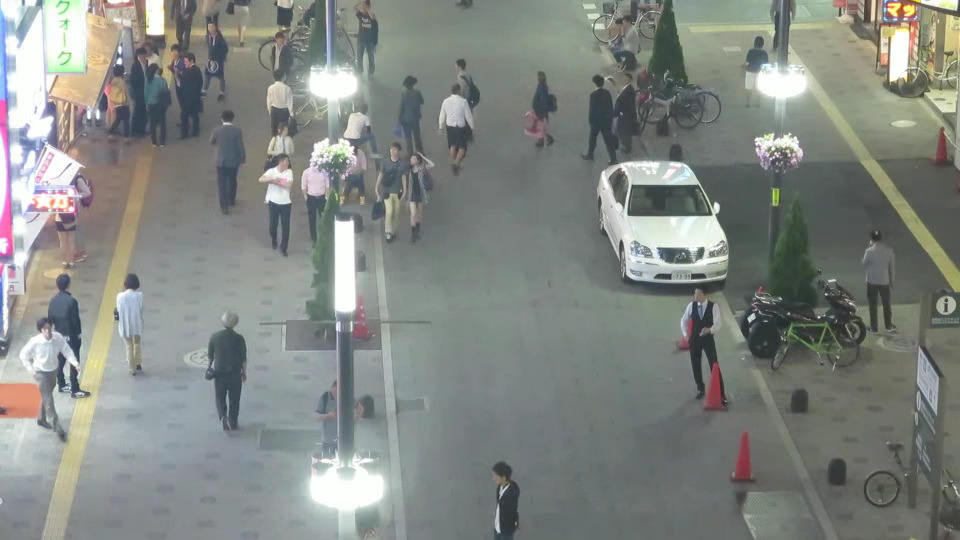
\includegraphics[height=3cm]{MOT16_sample}
    \caption{Example frame from the \cite{MOT16} dataset.}
    \label{fig:mot_sample}
\end{figure}

We have decided to create our dataset targeting the retail environment, as we have not found any usable data from the specified environment. Such a dataset will be more representative and allow for more accurate evaluation. Further, it can be used to optimize and fine-tune the system for the target environment. 

Dataset collection was done in cooperation with store owners, where the designed system might be used in the future. This cooperation allowed us to collect the dataset according to the system's assumed use. Collecting the dataset in the retail environment has shown some complications the system might face in actual usage and helped significantly with problem analysis from a practical standpoint.

The dataset collection process was done across two locations. The first location was used for selecting a camera, finding suitable camera placement, and initial experiments. The dataset itself was collected at the second location.

\subsection{Camera Selection}

This section describes the first part of the dataset collection process, where short videos were recorded with multiple cameras in different positions at the first location.

Cameras were placed in a shop window behind glass with the view facing the street. Evaluation criteria were image quality, camera view (does the camera see the full \gls{roi}), and camera noticeability. Camera noticeability is meant as a criterium of how much the camera is visible to a passerby, as a noticeable camera might discourage potential customers from browsing the shop window.

Three possible camera placement configurations were considered:
\begin{enumerate}
    \item at the edge of the shop window, near the glass, at approximately 150 cm from the ground,
    \item at the center of the shop window, near the glass, at approximately 150 cm from the ground,
    \item at the edge of the window in the corner, at approximately 220 cm from the ground, positioned at an angle.
\end{enumerate}

The first option did not present a sufficient view of the \gls{roi} and was rejected. The second option provided good image quality while being more noticeable. The third option proved to be very unobtrusive with a good view. However, the image quality seemed subjectively slightly lower, mainly thanks to reflections on the glass window.

Recordings from the second and third configurations were further evaluated using a simple initial version of the tracking algorithm. This early evaluation confirmed the third configuration as suitable and hinted at the task as being reasonably solvable. 

Based on the initial testing, the AXIS FA1105 surveillance camera\cite{axis_fa1105} was selected for the following recordings. This camera is highly discreet, provides sufficient video quality with resolution 1920x1080 (1080p), and has a wide $111\degree$ horizontal field of view.

\subsection{Dataset Acquisition}\label{s:dataset_acquisition}

Before starting the dataset collection itself, we needed to find a suitable camera configuration for the second location, which proved to be more challenging than expected. The camera was placed at a shop inside a shopping mall. The main difficulties were caused by camera obtrusiveness and appearance, lighting conditions, and reflections.

The camera appearance issue was solved by 3D printing a custom camera holder, which allowed for a more discrete and pleasant camera look. One of the main lighting problems was direct lighting from the shopping mall ceiling, which was handled by adding a black cover on top of the camera to shield it from this lighting. The camera is shown in figure \ref{fig:camera}.

\begin{figure}[ht]
    \centering
    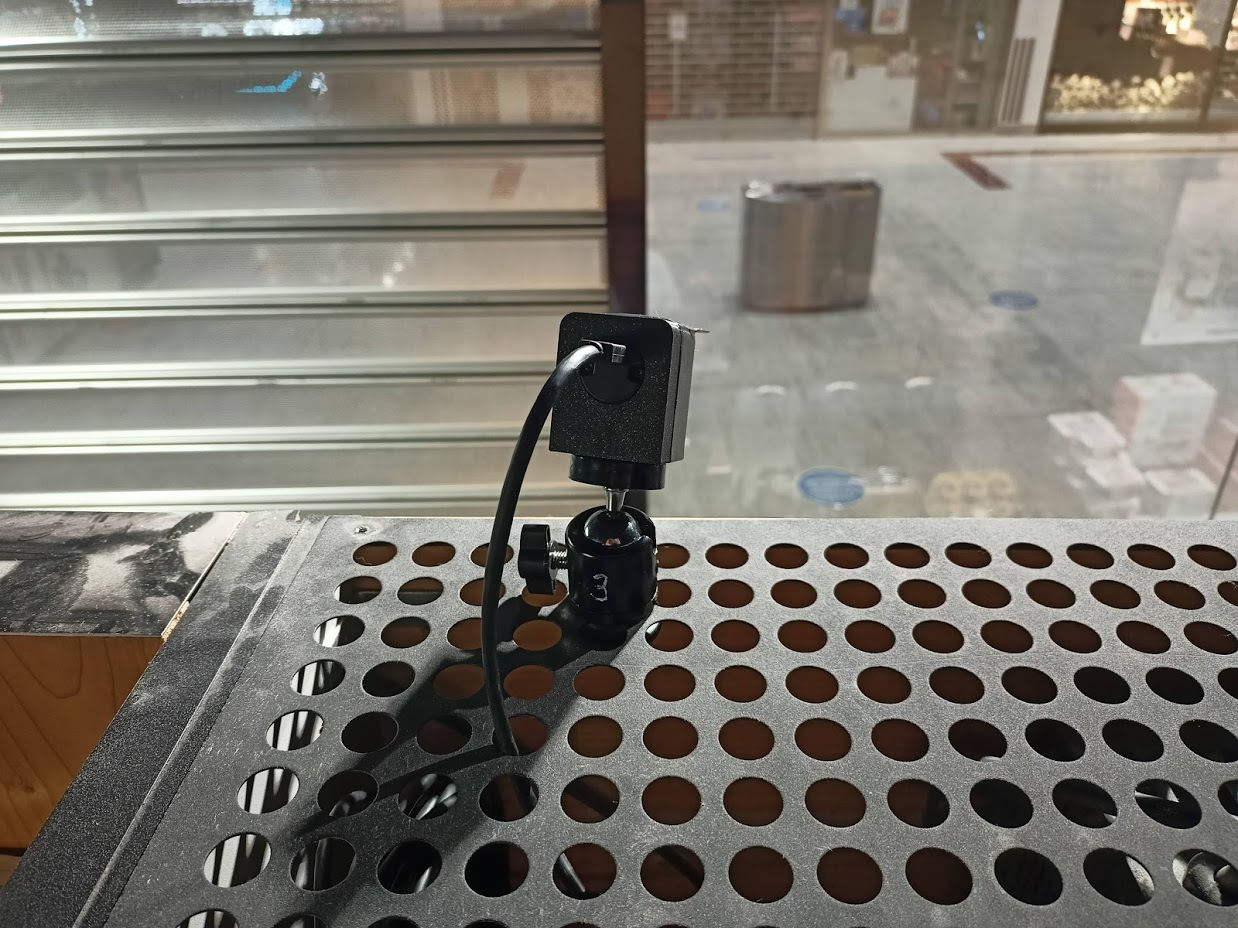
\includegraphics[width=5cm]{camera_back}
    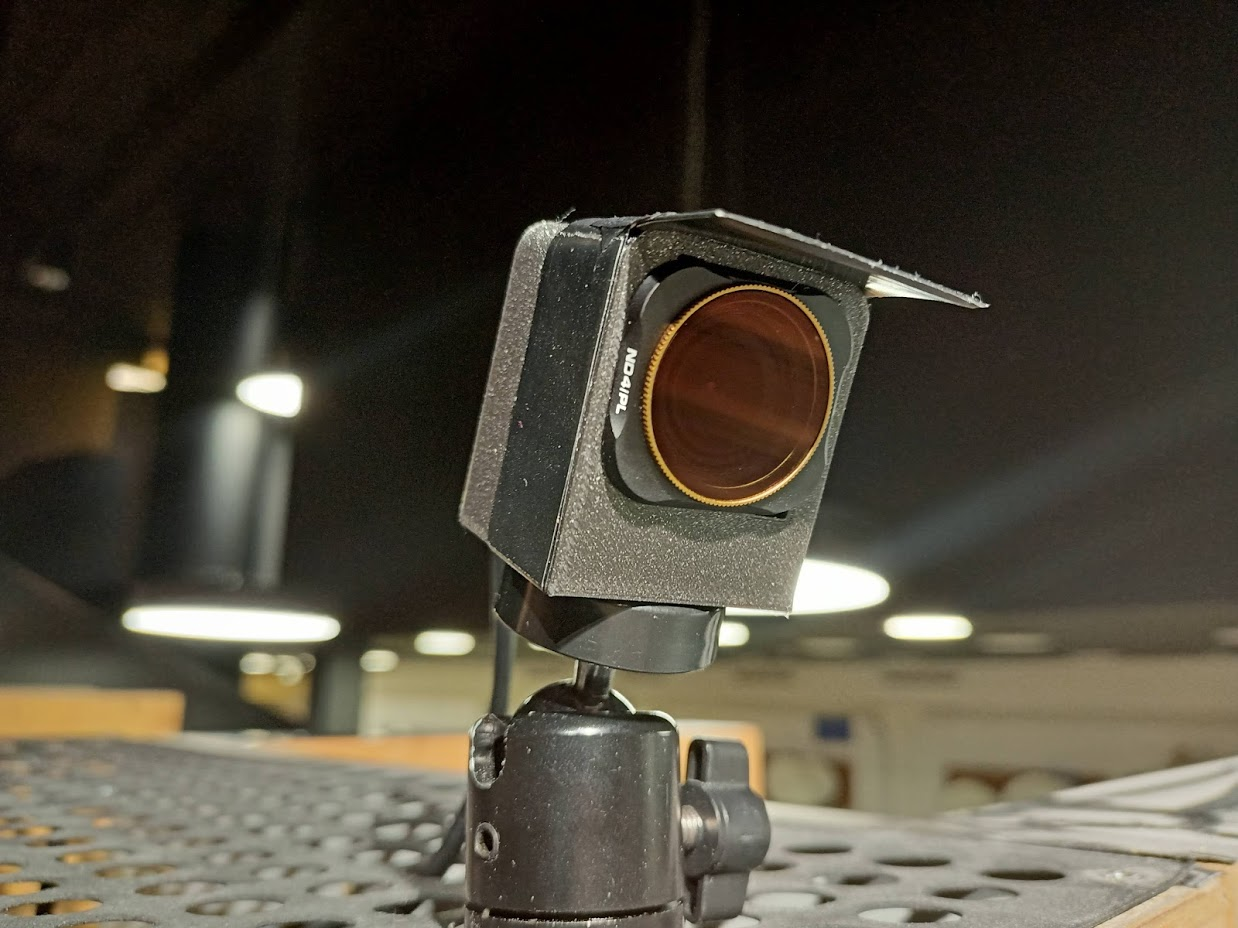
\includegraphics[width=5cm]{camera_front}
    \caption{Camera used for dataset acquisition.}
    \label{fig:camera}
\end{figure}

Another significant problem was reflections on the shops' glass windows. A polarization filter was added to the camera to minimize these reflections. While this improved the image quality, reflections remain a problem. The effect can be seen in figure \ref{fig:polarizer}.

\begin{figure}[ht]
    \centering
    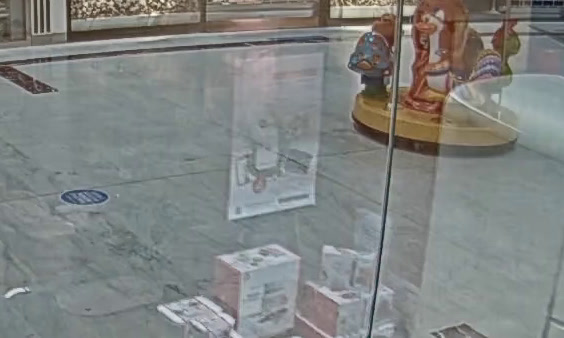
\includegraphics[width=5cm]{polarizer_bad}
    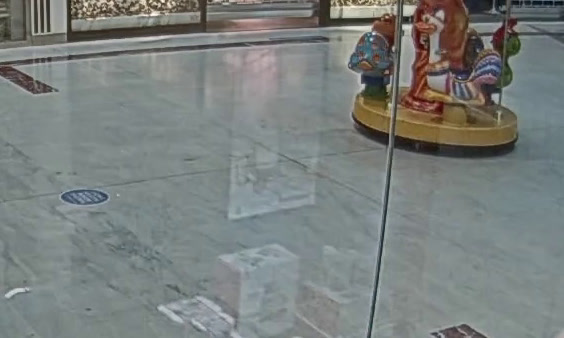
\includegraphics[width=5cm]{polarizer_good}
    \caption[Image taken without a polarizer filter and with polarizer filter.]{Image taken without a polarizer filter (left) and with polarizer filter (right).}
    \label{fig:polarizer}
\end{figure}

The camera remained in the location long-term, however usable dataset size is limited by the time needed to annotate the data. Multiple video sequences were hand-selected and annotated using CVAT software\cite{cvat}. The total dataset size is 2600 annotated frames. A sample dataset frame can been seen in figure \ref{fig:dataset_sample}.

\begin{figure}[ht]
    \centering
    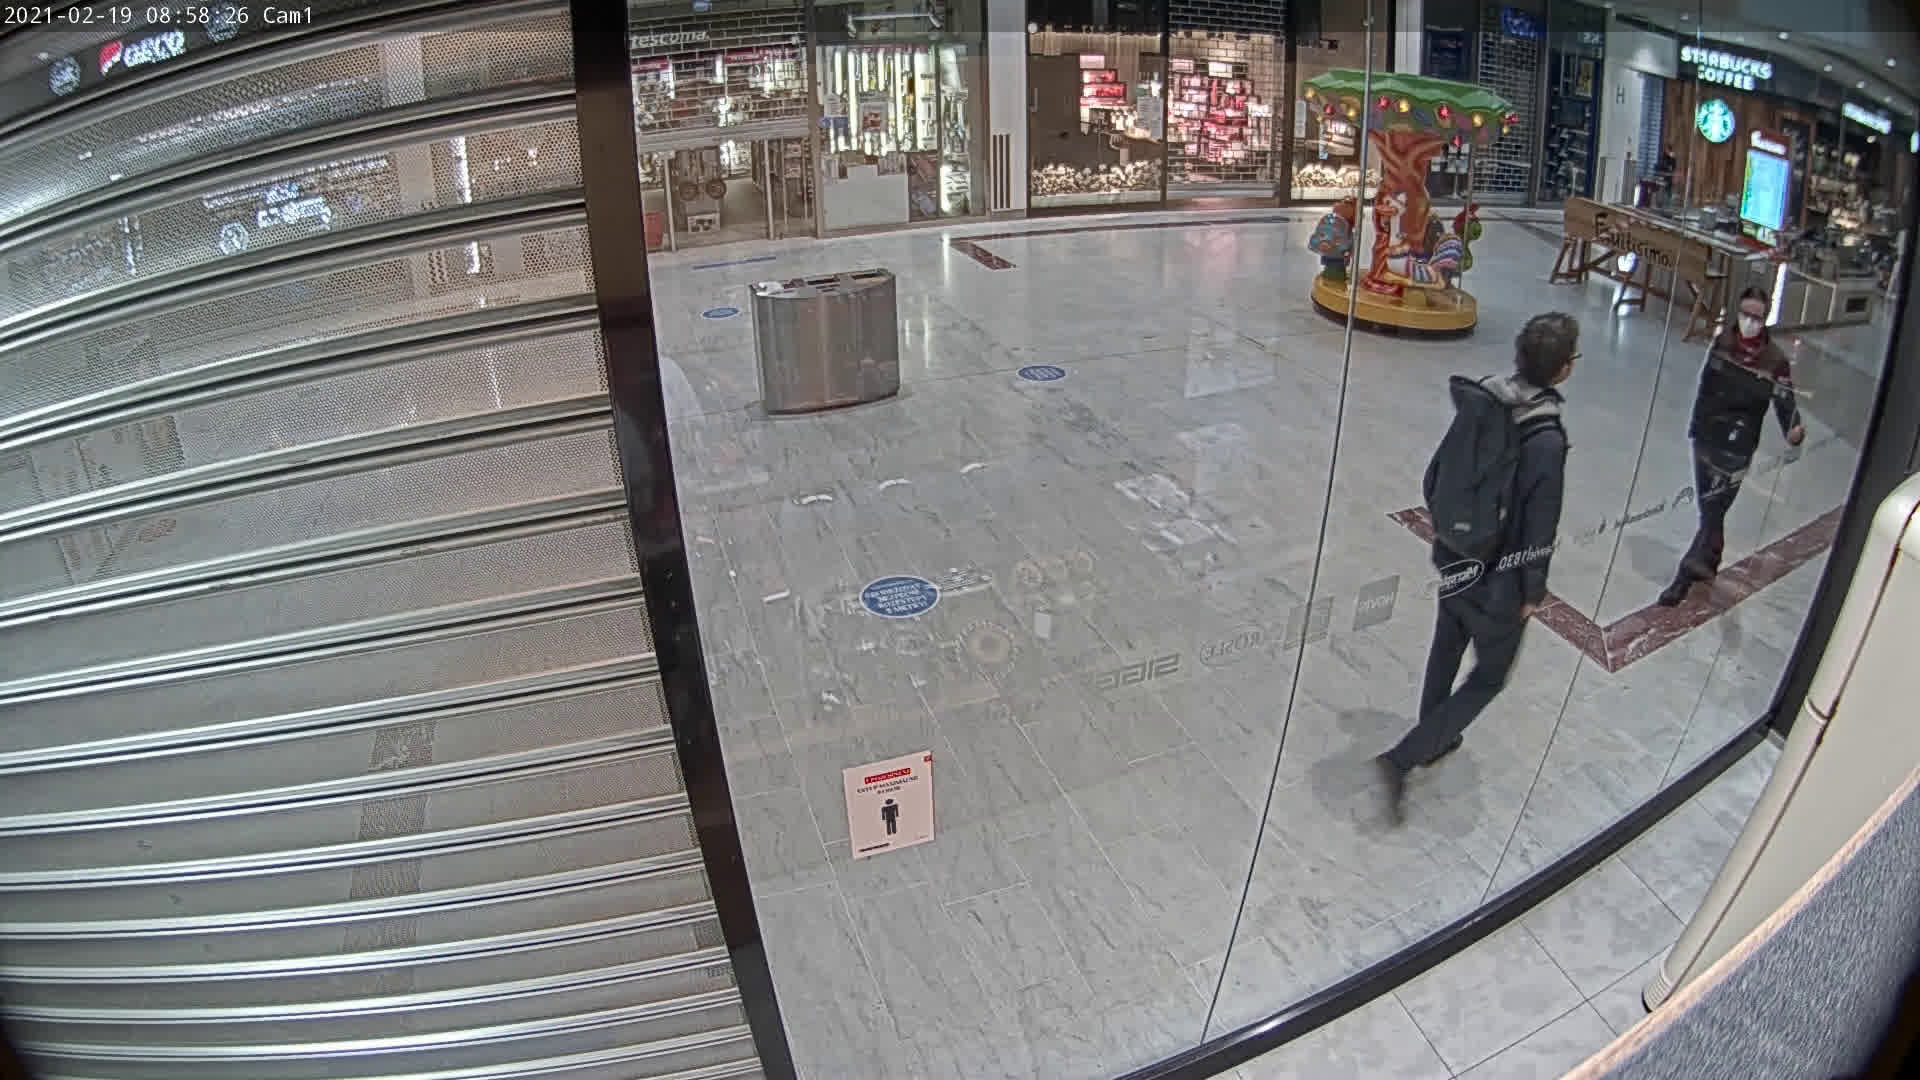
\includegraphics[width=8cm]{dataset_sample}
    \caption{Sample frame from collected dataset.}
    \label{fig:dataset_sample}
\end{figure}

\subsection{Region of Interest}

The goal of our work is to observe a region in front of a shop. It can be expected that the camera captures a larger area, as is the case in our collected dataset. The tracks need to be filtered based on their position to select only the tracks in the target area to provide relevant statistics.

The \gls{roi} is also relevant for the experimental evaluation. Evaluating tracks only in \gls{roi} makes the evaluation more relevant to the actual goal. Tracking people far away from the shop (and the camera) is not our goal and may not be reasonably achievable. Tracks in a significant distance are small, their image resolution is low, and occlusions and bounding box overlaps make this even more difficult. What is considered relevant needs to be considered for each camera setup individually.

To filter the relevant tracks, we need to specify a function to tell if a given track lies inside the \gls{roi}. The target area could be intuitively specified as a polygon. More general shapes could allow more flexibility but increase the complexity of operations such as intersection. Once we have the target area specified as some geometric shape, we can find if a track is inside based on bounding box intersection. Simple intersection could also be expanded to consider, for example, only tracks above some intersection over minimum threshold. Another possible approach is to convert each track to a single point (such as its bounding box center) and then find if the given point lies in the \gls{roi}.

The methodology used for evaluation is described in chapter \ref{ch:experiments}.

\subsection{Age and Gender Information}\label{s:dataset_age_and_gender}

The original goal for the dataset was to include age and gender information. This was an additional reason for collecting our dataset, as we do not know any \gls{mot} dataset that includes the biometric information. The current Covid-19 epidemic complicates the task significantly, as (nearly) all people wear face masks.

Initial experiments on collected data confirmed that extracting biometric information on images with face masks is challenging and currently available models and datasets are not sufficient for this task. Furthermore, we did not find any relevant datasets and little relevant work, which is probably caused by how unexpected and novel the current pandemic situation is.

Dealing with face masks properly is out of scope for this work. We consider the mask situation temporary, so it is not essential for future use of the application.

Based on the current difficult situation, we have made the following decisions. We do not include the age and gender information in our collected dataset. We include the age and gender classification in our pipeline; it is prepared for use once the situation with face masks changes. We evaluate the age and gender models mainly from the performance standpoint.

%%%%%%%%%%%%%%%%%%%%%%%%%%%%%%%%%%%%%%%%%%%%%%%%%%%%%%%%%%%%%%%%%%%%%%%%%%%%%%%%%%%%
\section{Age and Gender Classification}

% we want to extract age and gender -> use CNNs
One of the goals of this thesis is to extract age and gender information for tracked people. Multiple works dealing with this task exist, using various \gls{cnn} architectures\cite{levi2015age, yang2018ssr, karkkainenfairface}.

% you can use the same architecture for both tasks
The same network architecture can typically be used for both age and gender as in \cite{levi2015age}, except the last layer, which has to match the target number of classes.

% output
The expected output for gender is either male or female. For age information, the output format is less straightforward.

% output - classification vs regression
While age estimation has been formulated as a regression problem, for example, in \cite{yang2018ssr}\footnote{Even \cite{yang2018ssr} is based on classification that is turned into regression using expected values.}, it is more common to formulate it as a classification problem, where the categories are various age ranges\cite{levi2015age, karkkainenfairface}.

% output - use classification
Formulating the age prediction as a classification task into some age ranges simplifies the task (as we do not try to predict the exact age) and arguably does not reduce the information usefulness noticeably. Marketing strategies and behavior prediction will probably be different for various age groups, such as children, adults, and the elderly, but differ less inside these groups.

\subsection{Classification Input}

% input - body vs face
The required information can be extracted either from a whole-body image or from a face image. Using a whole-body image would be very beneficial since this information is always available, and no association step is needed. \cite{pavlakos2019expressiveBody} explores gender classification based on body pose estimation, which is in turn based on image information. We experimented briefly with this approach and found both performance and accuracy to be insufficient.

% input - face
A more typical approach is to use face information\cite{levi2015age, yang2018ssr, karkkainenfairface}, which has its own downsides. The face may not always be visible, and we need to associate faces to appropriate tracks.

% input - video (not single image)
In contrast to classification on a single image, our input is a sequence of frames. We need for a given face to be visible on at least one frame to make predictions. While this provides no guarantees, it makes the chance of a successful face detection more likely. If we have multiple predictions for a single track, we need to put them together using some statistical function such as mean or median.

\subsection{Face Alignment}

Both literature\cite{karkkainenfairface} and our experiments suggest that the classification task is heavily influenced by face alignment. We found that many detected faces are practically unusable for prediction because of alignment and general image quality issues.

As a potential improvement, we experiment with filtering faces based on face alignment. The goal is to accept predictions that are based only on face images with reasonable quality and alignment.

%%%%%%%%%%%%%%%%%%%%%%%%%%%%%%%%%%%%%%%%%%%%%%%%%%%%%%%%%%%%%%%%%%%%%%%%%%%%%%%%%%%%
\section{Hardware and Performance}

Most tracking and age and gender classification methods use \glspl{nn} as described in previous chapters. One of the limiting factors of \glspl{nn} is the computing power they require\cite{MOT16, yolo}.  Advances both in theoretical understanding and hardware have allowed for \glspl{nn} to be used in an increasing number of devices such as mobile phones\cite{mobilenets} and even browsers\cite{tfjs}.

However, video processing is still a very data-intensive task. Processing live feed requires processing multiple images each second. One of the system's primary goals should be to focus on speed to allow live camera feed processing.

Furthermore, using a dedicated (edge) device that would process the video stream at the camera's location would significantly improve the system's scalability and ease of use.

For these reasons, \gls{Jetson}\cite{jetson} was chosen as a testing device, which will be used to process the video stream and run the tracking algorithm in our experiments. This device is very compact and specialized for both video processing and \glspl{nn} inference, making it suitable for use in the retail environment. Running all experiments on single hardware assures that the results are comparable when looking at processing time. Running on a suitable device for the production environment also makes the results more directly relevant and usable.

\subsection{Optimization}

In recent years, there has been growing interest in building \gls{ai} models with the focus not only on quality but also on performance (computation power required)\cite{yukai_yang_2020_4294717_fastmot,tracktor_2019_ICCV,yolo}. Performance can often be significantly increased when using a smaller model\footnote{By smaller, we mean model with less learnable parameters. For \glspl{nn} the critical factor is typically depth; however, the overall architecture is also important.} without significant quality loss\cite{yang2018ssr}.

Another important topic is optimization of existing models. The task of reducing \gls{nn} size by removing parameters is called \textit{pruning}\cite{blalock2020stateOfPruning}.

A common pruning strategy\cite{blalock2020stateOfPruning} is to first train the target \gls{nn} to convergence. After which parameters or structural elements are issued a score. The network is then pruned based on these scores. Pruning typically reduces\footnote{Pruning can also increase the accuracy in some cases\cite{Molchanov_2019_CVPR_improtanceEstimationForPruning}.} the accuracy of the network, so the network can then be trained further (this is called \textit{fine-tuning}).

NVIDIA TensorRT\cite{vanholder2016efficientTensorRT} is a framework for \gls{nn} optimization and efficient inference. This software is closed-source, and the precise optimization algorithm is not disclosed. We will evaluate it experimentally in chapter \ref{ch:experiments}.
